\documentclass{article}
\usepackage[utf8]{inputenc}
\usepackage{soul, amsmath, listings, pdfpages}
\usepackage{graphicx}
\usepackage{tikz}
\usetikzlibrary{arrows.meta,positioning}

\newtheorem{theorem}{Theorem}
\newtheorem{corollary}{Corollary}[theorem]
\newtheorem{lemma}[theorem]{Lemma}
\newtheorem{definition}[theorem]{Defintion}

\lstset{language=Python}          % Set your language (you can change the language for each code-block optionally)

\usepackage[backend=biber,style=numeric,natbib=true]{biblatex} % Use the bibtex backend with the authoryear citation style (which resembles APA)

\addbibresource{References.bib} % The filename of the bibliography

\title{INF5870 - First Mandatory Assignment}
\author{Zahra G. Yndestad \\ Khalil Abuawad \\ Marius E. G. Andresen \\ Christopher A. Trotter}
\date{February 2017}

\begin{document}

\maketitle

\section{Question 1}
	Since the question can derive multiple examples that lead to the same optimal minimum, depending on the assumptions made, we have decided to give a time frame for when these shiftable appliances can run and we shall attempt to cover all possible cases. Since all of the mentioned appliances for the home are shiftable, then providing examples of different setup times and deadlines would be redundant. We will rather assume that the total runtime of each appliance is less than 20 hours. Giving us that each appliance can be completed within the off-peak hours. Also, in the assignment we are provided the daily cost of these various appliances which differs from non-shiftable appliances, for example: the light bulb. Allowing us to suggest any time span that meets the daily consumption.  As a condition, each of the appliances has to have their runtime outside the peak hours to achieve the optimal minimum. Any example which provides the optimal minimum will have to respect this condition, regardless of the strategy. We will provide a general definition of a strategy, then discuss what is a reasonable strategy.

	\begin{definition}
    	A strategy is a high level plan to achieve one or more goals under conditions of uncertainty{\cite{wikistrategy}}.
	\end{definition}

	From our assumptions above, we can assume our strategy is trivial in the sense that all the appliances can be run in the off-peak hours. Secondly, any of the strategies can deviate from having all appliances running at the same time, centralized, to running them sequentially in some order, distributed. From these different perspectives of strategies, we can now discuss what is a reasonable strategy by first defining Demand and Response and after taking into consideration general issues of Demand and Response.

	\begin{definition}
	    Demand Response Management (DRM) is defined as changes in electric usage by end‐use customers from their normal consumption patterns in response to changes in the price of electricity over time, or to incentive payments designed to induce lower electricity use at times of high wholesale market prices or when system reliability is jeopardized\cite{defDRM}.
	\end{definition}


	As an assumption to the question, the customer is to be incentivised based on the electrical pricing scheme known as \emph{Time-Of-Use (ToU)}. Meaning that the customer is informed ahead of time about the price of electricity. Assuming that this will result in users using less electricity when electricity prices are high.

	We are now left with discussing a reasonable strategy that respects the assumptions. These assumptions are there to help provide a way to achieve one or more goals under conditions of uncertainty, which is the definition of a strategy. Other strategies that do not respect the assumptions are trivially unreasonable. Since all the strategies that respect the assumption are by themselves reasonable, it is important to differentiate between weakly and strongly reasonable strategies. Differentiating these strategies can simply be done by understanding the conditions of uncertainty. Less uncertainty can relate to a strongly reasonable strategy, and weakly reasonable as the opposite.

	Now to bring this all into context, a centralized strategy would mean that all appliances are run at the same time which could potentially cause the pricing scheme to change over time. Making this to be a weakly reasonable strategy because it maintains a high level of uncertainty by creating new peak hours. On the other hand, we have a decentralized strategy that would run all appliances after each other in some order. In this case we would have a strongly reasonable strategy by the fact that the pricing scheme would be unchanged and the probability of occurring peaks would be highly unlikely. Giving us that the most reasonable strategy would be to start different appliances after each other in some order.

	For our solution of a strategy in Question 1, we have used Linear Programming, LP, solver in R to determine our strategy. In a realistic application, this would provide us with the strongly reasonable strategy of distributing the applications based on the hourly consumption to meet the daily consumption. Since we are to provide our own examples and define our own assumptions, we can conclude that our resulting strategy is a hybrid between strongly and weakly strategies.

\newpage

	\section{Question 2 and 3}
	Since both question 2 and 3 from the assignment have almost the same requirements it seemed sensible to cover both of them under the same section. The comparative analysis of question 3 has been done in a separate section. To begin with, we shall explain the algorithm of our solution and then provide a flow diagram showing the algorithm.

	%The formulation of the demand response as an optimization problem, e.g., linear programming problem. Please use a figure to show the pricing curve. Please explain on how the problem is solved and probably draw the flowchart to illustrate the main algorithm(s).\\

	%%%%%%%%%%%%%%%%%%%%%%%%%%%%%
	% Emi wrote here, start:    %
	%%%%%%%%%%%%%%%%%%%%%%%%%%%%%

    %\newline \noindent We divided the program into two files, one handling lp (DRM.R) and the other handling the preparations of data and plotting (Assignment\_1.R). \\

    %\newline \noindent In Assignment\_1.R we start by generating both price schemes used, Time-of-Use (ToU) and Real-Time-Pricing (RTP). Then we read in two predefined csv files containing the appliances used for the simulation. We decided to answer all the questions in one file, but divided each question into their own respective function so that they could easily be called individually, but for simplicity we call them all in order and print the results two the console. Each function select the date requested by the question, then call DRM with the selected price scheme and the data set containing the chosen appliances. The function then returns the dataset recieved by DRM.\\

    %\newline \noindent DRM.R consists of the funtion DRM. DRM contains all the necessities to compute lp. It takes in two parameters, the chosen price scheme and a data set including all appliances for the computation. It then generated the needed matrices; constraints, usage, price and operators. Then it will proceed to call lp with the generated matrices and return the data set returned by lp.\\

    %%%%%%%%%%%%%%%%%%%%%%%%%%%%%
	% Emi wrote here, end.      %
	%%%%%%%%%%%%%%%%%%%%%%%%%%%%%

	\subsection{File structure}
	We have divided the assignment into two files, Assignment\_1.R and DRM.R, where the first file creates each question as a function and formats the parameters to be used in the second file. The second file is the Linear Programming (LP) solver itself and the way we have chosen to structure the input for the LP-solver. Our program is initialised from the first file.

	\subsection{Reading the data files }
	As the program initializes, the pricing schemes ToU and RTP are created, and the program reads in two different comma separated (.csv) files. The .csv files contains a list of appliances together with their daily and hourly usage and earliest and latest start time. The first file contains the fundamental appliances, provided in the assignment, while the other file contains random appliances that are arbitrarily selected. Our simulation of multiple household is based on the first file and then continuously selecting arbitrary random appliances from the second file to differentiate the households in the neighbourhood.

%	At the start of the program the pricing schemes ToU and RTP are created, and then the program reads the .csv data file. This data file contains a list of appliances and their daily usage, hourly usage, earliest and latest time of use. This data set is supposed to reflect the fundamental appliances in a standard household. We also have a list of random appliances, similar to previous mentioned list, which is supposed to show what some households in given neighbourhood could possibly contain.

	\subsection{Generation of data set}
	After reading the data file, the program will continue by generating a data set that consists of both shiftable and non-shiftable appliances, and even append some random appliances which in our case are only shiftable. To differentiate between shiftable and non-shiftable we have given that if the hourly consumption multiplied with the total time run is equivalent to the daily usage, then it is shiftable. In the case of non-shiftable it is greater than the daily usage.


	\subsection{Making the matrices}
	To be able to use the LP-solver, we have to format the input such that we can format the daily and hourly usage constraints with the given pricing scheme. As part of the formatting it required us to generate a matrix which was provided information from the data set. With the pricing scheme and this matrix we were able to generate an instance of the LP-solver which in returned the optimal minimum cost.

	\subsection{Pricing Curve}
    Below is shown the two different pricing schemes which determined the pricing curve for question 1, 2 and 3.
    \begin{figure}[ht]
    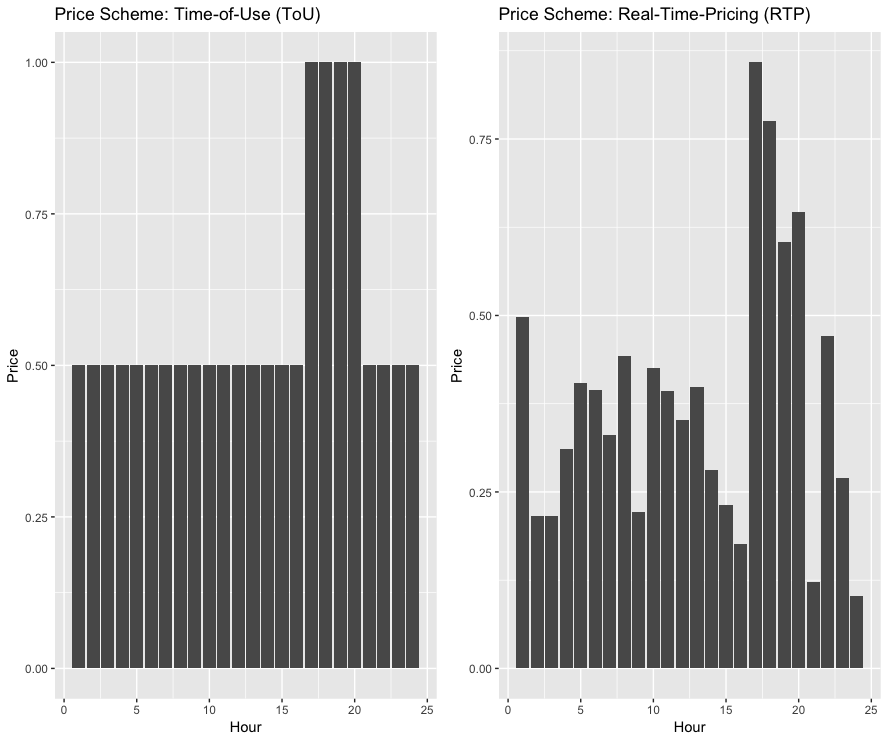
\includegraphics[scale=0.3]{pricing_schemes.png}
    \centering
    \end{figure}

\newpage

    \subsection{Flow Chart of algorithm}
    Below is shown the flow chart describing the flow of the algorithm. Note: the thick parallel bar in this instance shows that question 1, 2 and 3 are run sequentially, but can also be run independently. Furthermore, we could have provided a flow chart of how the input of the LP-solver is formatted, but for convenience we have abstracted this away.

     \begin{figure}[ht]
    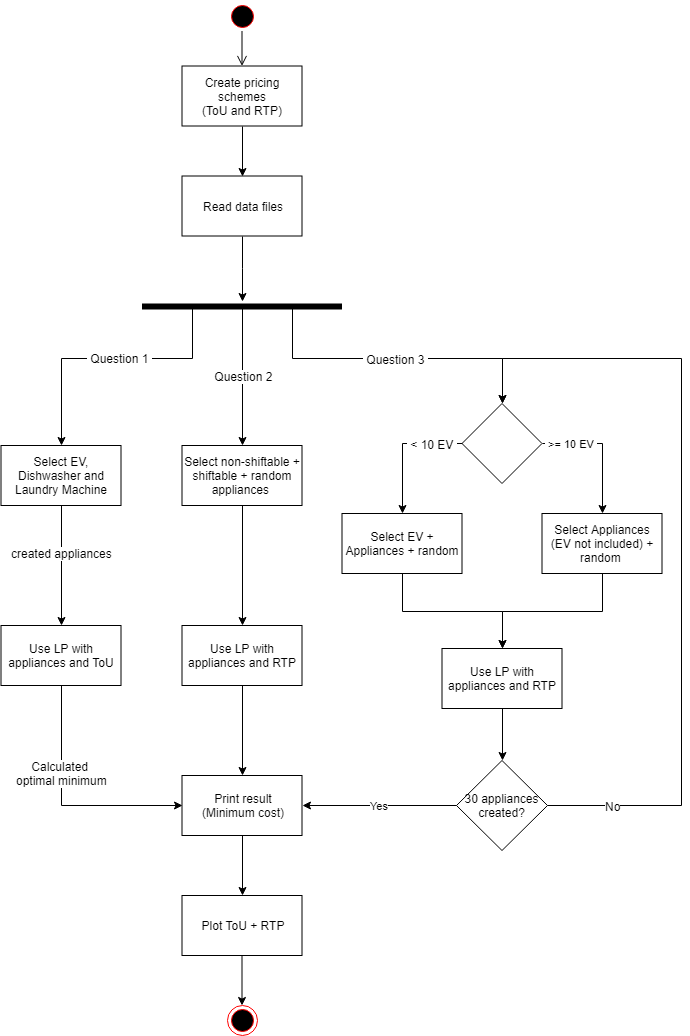
\includegraphics[scale=0.4]{flowChart.png}
    \centering
    \end{figure}




\newpage

    \section{Pricing scheme comparative analysis}
        Briefly introduced in Question 1, of the report, was the pricing scheme \emph{Time-of-Use (ToU)}, which we will compare with a different pricing scheme, used in the assignment, known as \emph{Real-Time-Pricing (RTP)}. RTP normally changes the cost of electricity from hour to hour. Commonly, most consumers are forced to pay the same price no matter the electricity, but real-time-pricing lets consumers adjust their electricity usage accordingly; for example, scheduling usage during periods of low demand to pay cheaper rates.

        In regards to the analysis, it is often done in correlation with real data sets provided to assess the validity of the conclusion and evaluation of the research. As the data sets created in the assignment are mere assumptions it does not provide a fundamental basis for the analysis. We will rather analyse the pricing schemes based on their practicality in a sub-realistic context of how adaptive they have become and in what use cases they might be relevant. Also, our analysis has been influenced by a comparative research of these pricing schemes done in \cite{RTPvsToU}.

        %As we can recall, ToU has a set period where the consumer is aware of the pricing of electricity and this is usually known well in advance of the period.

        An important factor to take into account is that these pricing schemes are marginal costs that should benefit over time. Which means that the data of the analysis should be acquired from a set period of time such as a few months, or even years. Our goal for the analysis is to optimize the marginal cost and evaluate what pricing scheme achieves this.

        As we can recall, ToU has a set period where the consumer is aware of the pricing of electricity and this is usually known well in advance of the period. It is an attempt to forecast the supply by adjusting the price of peak and off-peak periods. As this is an improvement of \emph{fixed rates (FR)}, it is still important to assess the potential marginal cost loss when a forecast is done far ahead of time. In contrary, RTP does not require a forecast rather  it reflects the price based on the supply to circumvent extreme peaks in periods of high demand and low supply, but also provides an opportunity to acquire a significant amount of the supply for a small sum in periods of low demand and high supply. The overall goal of RTP is to equalise the difference of the supply and demand.

        Already from introducing these two pricing schemes we can assess that RTP is the most efficient method to optimize the marginal cost, but this comes with a certain amount of risk. Since the price is reflected based on the supply, it has a volatility applied to the scheme which can be viewed as a high risk and high reward factor. Where as with a fixed rate, it is ensured that the price will remain the same regardless of the supply. ToU is a scheme which compliments these two, but is required to be adjusted in such a way to balance the trade-off between risk, reward, safety and security. If ToU rates are set much in advance, and fixed over the hours, these rates miss the majority of the potential gain as measured by the variance index shown in \cite{RTPvsToU}. This indicated that there is a substantial difference in efficiency between even the best ToU design and RTP. Meaning that their is required further work to balance the trade-offs mentioned to find a suitable pricing scheme. As of now, where real-time pricing is available it seems worth the effort to make adjustments from going all the way to RTP. Giving that a hybrid pricing scheme which is between the best ToU design and RTP is required to balance the marginal cost optimization with the given trade-offs.

    \printbibliography[heading=bibintoc]
\end{document}
